\begin{frame}
  \frametitle{\problemtitle}
  \begin{block}{Problem}
    You are given a graph consisting of line segments in 3D space.
    You travel on a ship with constant acceleration and constant fuel consumption for the time spent accelerating.
    You need to come to a standstill at each vertex.
    Given a target location and a time limit, find the minimum amount of fuel needed to get there.
    You need to answer multiple queries, all from the same starting location.
  \end{block}
  \begin{center}
    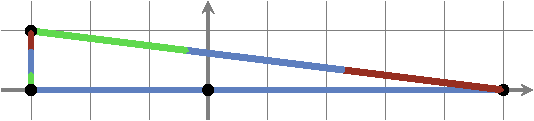
\includegraphics[width=0.7\textwidth]{sample1}
  \end{center}
\end{frame}
\begin{frame}
  \frametitle{\problemtitle}
  \begin{block}{Solution for fixed path}
    \begin{itemize}
      \item Consider a path consisting of multiple line segments.
      \pause
      \item Suppose the $i$th segment is $d_i$ metres long and we accelerate/decelerate for $x_i$ seconds along it.
      \item Then it takes $x_i + \frac{d_i}{x_i}$ seconds to traverse the $i$th segment.
      \item New problem: minimize $\sum 2x_i$ subject to $\sum x_i + \frac{d_i}{x_i} \le t$.
      \item \textbf{Key insight}: optimum is reached when $x_i = c\cdot\sqrt{d_i}$ for some constant $c$.
      \item We can compute $c$ by solving $c + \frac{1}{c} = t / \sum\sqrt{d_i}$. When the RHS is $< 2$, no solution exists.
    \end{itemize}
  \end{block}
  \pause
  \begin{block}{Solution}
    \begin{itemize}
      \item<+-> To keep the time limit and save fuel, find a path that minimizes $\sum\sqrt{d_i}$.
      \item<+-> Use Dijkstra's algorithm for this, where edges have length $\sqrt{d_i}$.
      \item<+-> The starting location is fixed, so queries can be answered in constant time.
    \end{itemize}
  \end{block}
  \solvestats
\end{frame}
